\subsection{Aufgabe 3}
\begin{figure}[H]
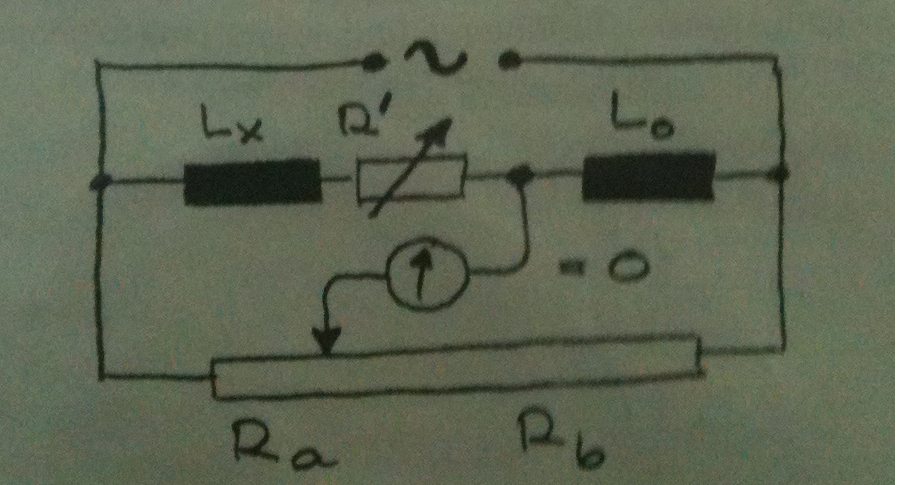
\includegraphics[scale=0.5]{sb3}
\caption{Abbildung 1: Schaltplan Aufgabe 3}
\end{figure}
In der letzten Aufgabe wurde eine Wechselstrombrücke aufgebaut um nun die Induktivität L einer Spule zu bestimmen. Der Aufbau besteht aus einem Phasenabgleichswiderstand R' mit einer bekannten und einer unbekannten Spule \(L_{0}\) und \(L_{x}\) in Reihe geschalten und dazu parallel ist die Wechselstrombrücke. Das Messgerät wird zwischen R' und der Wechselstrombrücke platziert. Das Ziel ist nun eigentlich, den Strom durch die Wechselstrombrücke auf Null zu stellen, was allerdings wegen den hier verwendeten Bauteilen nicht ganz möglich ist. Also versucht man ihn zu minimieren. Gemessen hatten wir mit dem Messgerät ELC-131D (\(\pm 2\% +5\) dgt) für \(\Delta L_{VS}\) und (\(\pm 0,5\% +3\) dgt) für \(\Delta R_{VS}\)\\
Bei einer Frequenz von f=1.9989 kHz erhielten wir für die gesuchten Größen folgende Werte:
\\

\begin{tabular}{l l}
\(R_{a}\) & =\(761,0\pm 4,3 \Omega\)\\
\(R_{b}\) & =\(241,8\pm 1,7 \Omega\)\\
\(R'\) & =\(3,700\pm 0,023 \Omega\)\\
\end{tabular}
\\

Für die Vergleichsspule gelten die Werte:\\

\begin{tabular}{l l}
\(R_{VS}\) =\((2,91\pm 0,02)\Omega\)\\
\(L_{VS}\) =\((1,507\pm 0,015)\)mH\\
\end{tabular}
\\

Nun überprüftt man mit dem Oszilloskop, ob die Spulen mit dem Funktionsgenerator in Phase sind.\\
\newpage
Des weiteren gilt es nun die Induktivität L und den Verlustwiderstand \(R_{V}\) der unbekannten Spule berechnen. Dazu nimmt man Gl.\(\eqref{L}\) für \(L_{x}\):
\begin{equation}\notag
L_x = {\frac{R_a}{R_b}} L_0=(4,75\pm 0,07)mH
\end{equation}

und auf Grund der Phasengleichheit errechnet sich für \(R_{V}\):
\begin{equation}\notag
R_{V}=\frac{R_{a}}{R_{b}}\cdot R_{VS}=(9,16\pm 0,11)\Omega
\end{equation}
Für die Fehler gilt:
\begin{equation}\notag
\Delta L_x = {\sqrt{\left({\frac{\partial L_x}{\partial R_a}}\Delta R_a\right)^2+\left({\frac{\partial L_x}{\partial R_b}}\Delta R_b\right)^2+\left({\frac{\partial L_x}{\partial L_0}}\Delta L_0\right)^2}}
\end{equation}
\begin{equation}\notag
\Delta R_{L_x} = {\sqrt{\left({\frac{\partial R_{L_x}}{\partial R_a}}\Delta R_a\right)^2+\left({\frac{\partial R_{L_x}}{\partial R_b}}\Delta R_b\right)^2+\left({\frac{\partial R_{L_x}}{\partial R_{L_0}}}\Delta R_{L_0}\right)^2}}
\end{equation}
\\

Als letztes wird noch der theoretische Werte für den Phasenunterschied bestimmt. Gemessen hatten wir für die Induktivität L:
\begin{equation}\notag
L=(4,823 \pm 0,038)mH
\end{equation}
\begin{equation}
\notag
R_{L}=(162,5 \pm 1,3)\Omega
\end{equation}

Dies nun in Gl.\(\eqref{d}\) eingesetzt mit \(\omega=2\pi f\) (f=199,98 Hz) und nach \(\phi\) aufgelöst, ergibt:
\begin{equation}
\notag
\phi=arctan \left(\frac{2\pi f L}{R_{L}}\right)=(2,14 \pm 0,03)^\circ
\end{equation}

Für den Fehler gilt wieder:
\begin{equation}\notag
\Delta \phi = {\sqrt{({\frac{\partial \phi}{\partial R_{L_1}}}\Delta R_{L_1})^2+({\frac{\partial \phi}{\partial L_1}}\Delta L_1)^2}}
\end{equation}

\subsection*{Fazit}
An sich verlief bei dieser Aufgabe alles soweit ganz gut, bis auf das kleine Zeitproblem was alle Gruppen bei diesem Versuch hatten. Da wir auch die einzige Gruppe waren, die den Aufbau zu dieser Aufgabe geschafft hatten, durften wir sozusagen den Versuch vorführen. Das ging dann allerdings ein wenig chaotisch zu, weil immer nachgefragt wurde was jetzt nochmal welcher Wert genau gewesen war. Nichts desto trotz sehen unsere Ergebnisse für Diesen Versuch ganz ordentlich aus. Das einzige was komisch ist, ist dass unser Widerstand der Vergleichsspule so klein ist. Da uns aber Vergleichswerte fehlen, beruht diese Aussage eher auf ein Bauchgefühl, als auf Tatsachen.\\
In der Berechnung des Fehlers der Phasenverschiebung haben wir den Fehler für die Frequenz weggelassen, weil er im Verhältnis zu denen der anderen Werte so verschwindend gering ist, dass es nicht ins Gewicht gefallen wäre.\\
Alles in allem verlief dieser Versuch zufriedenstellend.